\documentclass{article}

\usepackage[italian]{babel}
\usepackage[margin=2cm, footskip=5mm]{geometry}
% questi package non sono necessari in lualatex; ref https://tex.stackexchange.com/a/413046
% \usepackage[utf8]{inputenc}
% \usepackage[T1]{fontenc}
\usepackage{enumitem}
\usepackage{hyperref}
\usepackage{titlesec}
\usepackage{soulutf8}
\usepackage{contour}
\usepackage{float}
\usepackage{graphicx}
\usepackage{fancyhdr}
\usepackage{longtable}
\usepackage[table]{xcolor}
\usepackage{titling}
\usepackage{lastpage}
\usepackage{ifthen}
\usepackage{calc}
\usepackage{minted}
\usepackage{pgfgantt}
\usepackage{subfiles}

\newlength{\imgwidth}

\newcommand\scalegraphics[1]{%
    \settowidth{\imgwidth}{\includegraphics{#1}}%
    \setlength{\imgwidth}{\minof{\imgwidth}{\textwidth}}%
    \includegraphics[width=\imgwidth]{#1}%
}

% XXX definizione dei percorsi in cui cercare immagini
\graphicspath{ {./}
    {./img/}
}

% esempio di utilizzo: \appendToGraphicspath{./img/} (un comando diverso per ogni path da includere)
% N.B.: ci DEVE essere un forward slash alla fine del path, a indicare che è una cartella.
\makeatletter
\newcommand\appendToGraphicspath[1]{%
  \g@addto@macro\Ginput@path{{#1}}%
}
\makeatother

% setup della sottolineatura
\setuldepth{Flat}
\contourlength{0.8pt}

\newcommand{\uline}[1]{%
  \ul{{\phantom{#1}}}%
  \llap{\contour{white}{#1}}%
}

% setup dei link
\hypersetup{
  colorlinks=true, % set true if you want colored links
  linktoc=all,     % set to all if you want both sections and subsections linked
  linkcolor=black, % choose some color if you want links to stand out
}

% setup di header e footer
\pagestyle{fancy}

\fancyhf{}
\fancyhead[L]{\includegraphics[width=1cm]{logo.png}}
\fancyhead[R]{\thetitle}
\fancyfoot[R]{\thepage\ di~\pageref{LastPage}}

\fancypagestyle{nopage}{%
  \fancyfoot{}%
}

\setlength{\headheight}{1.2cm}

% setup forma \paragraph e \subparagraph
\titleformat{\paragraph}[hang]{\normalfont\normalsize\bfseries}{\theparagraph}{1em}{}
\titleformat{\subparagraph}[hang]{\normalfont\normalsize\bfseries}{\thesubparagraph}{1em}{}

% setup profondità indice di default
\setcounter{secnumdepth}{5}
\setcounter{tocdepth}{5}

% shortcut per i placeholder
\newcommand{\plchold}[1]{\textit{\{#1\}}} % chktex 20

% hook per lo script che genera il glossario
\newcommand{\glossario}[1]{\underline{#1}\textsubscript{g}}

% definizione dei comandi \uso e \stato
\makeatletter
\newcommand{\setUso}[1]{%
  \newcommand{\@uso}{#1}%
}
\newcommand{\uso}{\@uso}

\newcommand{\setStato}[1]{%
  \newcommand{\@stato}{#1}%
}
\newcommand{\stato}{\@stato}

\newcommand{\setVersione}[1]{%
  \newcommand{\@versione}{#1}%
}
\newcommand{\versione}{\@versione}

\newcommand{\setResponsabile}[1]{%
  \newcommand{\@responsabile}{#1}%
}
\newcommand{\responsabile}{\@responsabile}

\newcommand{\setRedattori}[1]{%
  \newcommand{\@redattori}{#1}%
}
\newcommand{\redattori}{\@redattori}

\newcommand{\setVerificatori}[1]{%
  \newcommand{\@verificatori}{#1}%
}
\newcommand{\verificatori}{\@verificatori}

\newcommand{\setDescrizione}[1]{%
  \newcommand{\@descrizione}{#1}%
}
\newcommand{\descrizione}{\@descrizione}

\newcommand{\setModifiche}[1]{%
  \newcommand{\@modifiche}{#1}%
}

\newcommand{\modifiche}{\@modifiche}

\makeatother

% setup delle description
\setlist[description,1]{font=$\bullet$\hspace{1.5mm}, labelwidth=* leftmargin=*,labelindent=12.5mm}
\setlist[description,2]{font=$\bullet$\hspace{1.5mm}, leftmargin=*,labelindent=12.5mm}

\appendToGraphicspath{../../commons/img/}

\title{Verbale esterno --- 03/01/2020}

\setResponsabile{Alessandro Rizzo}
\setRedattori{Alberto Cocco}
\setVerificatori{
  Tobia Apolloni \\ &
  Riccardo Cestaro
}
\setUso{Esterno}
\setDescrizione{Verbale dell'incontro di GruppOne del 09/01/2020}
\setModifiche{%
\cellcolor{white!80!lightgray!100} &Alessandro Rizzo & 2020--01--10 & approva documento \\%
\cellcolor{white!80!lightgray!100} &Tobia Apolloni, Riccardo Cestaro & 2020--01--10 & verifica verbale \\%
\multirow{-3}{*}{-} \cellcolor{white!80!lightgray!100} &Alberto Cocco & 2020--01--09 & stendi verbale %
}

\disabilitaVersione{}
\disabilitaElencoFigure{}
\disabilitaElencoTabelle{}

\begin{document}

\thispagestyle{empty}
\pagenumbering{gobble}

\begin{center}

  \includegraphics[width=8.5cm]{\commons/img/logo.png}\\
  {\Large GruppOne - progetto "Stalker"}\\
  \vspace{1.5cm}

  {\Huge \thetitle}
  \vspace{1.5cm}

  \begin{table}[H]
    \centering

    \begin{tabular}{r|l}
      \textbf{Versione}     & \versione              \\
      \textbf{Approvazione} & \responsabile          \\
      \textbf{Redazione}    & \redattori             \\
      \textbf{Verifica}     & \verificatori          \\
      \textbf{Stato}        & \stato                 \\
      \textbf{Uso}          & \uso                   \\
      \textbf{Destinato a}  & Imola Informatica      \\
                            & GruppOne               \\
                            & Prof. Tullio Vardanega \\
                            & Prof. Riccardo Cardin  \\
    \end{tabular}
  \end{table}

  \vspace{3cm}
  \textbf{Descrizione}\\
  \descrizione\\
  \vfill
  \verb|gruppone.swe@gmail.com|
\end{center}

\newpage
\thispagestyle{nopage}

\section*{Registro delle modifiche}
\label{sec:registro_delle_modifiche}

\begin{table}[H]
  \label{tab:registro_delle_modifiche}

  \centering
  \rowcolors{2}{lightgray}{white!80!lightgray!100}

  \begin{longtable}[c]{c c c c l}
    \rowcolor{darkgray!90!}\color{white}{\textbf{Versione}} & \color{white}{\textbf{Data}} & \color{white}{\textbf{Nominativo}} & \color{white}{\textbf{Ruolo}} & \color{white}{\textbf{Descrizione}} \\\endhead
    \modifiche
  \end{longtable}
\end{table}

% section registro_delle_modifiche (end)
\newpage

\thispagestyle{nopage}
\pagenumbering{roman}
\tableofcontents

\newpage

\pagenumbering{arabic}


\section{Informazioni logistiche}%
\label{sec:informazioni_logistiche}

\begin{description}
  \item [Luogo] Torre Archimede, studio del prof. Tullio Vardanega
  \item [Data] 09/01/2020
  \item [Ora] 12:15 \symbol{8594} 14:15
\end{description}

\subsection{Membri del gruppo presenti}%
\label{sub:membri_del_gruppo_presenti}

\begin{enumerate}
  % \item Riccardo Agatea
  % \item Tobia Apolloni
  \item Riccardo Cestaro
  \item Alberto Cocco
  \item Luca Ercole
  \item Alberto Gobbo
  \item Alessandro Rizzo
  % \item Fabio Scettro
\end{enumerate}
% sub:membri_del_gruppo_presenti (end)

\subsection{Altri partecipanti}%
\label{sub:altri_partecipanti}
\begin{enumerate}
  \item prof. Tullio Vardanega (committente del progetto)
\end{enumerate}

% sub:altri_partecipanti (end)
% sec:informazioni_logistiche (end)

\section{Introduzione}%
\label{sec:introduzione}

La riunione si è svolta sotto forma di discussione: ogni componente del gruppo ha inserito in un file Google docs condiviso le domande a cui il committente ha successivamente risposto. Segue una descrizione degli argomenti trattati.

\section{Ordine del giorno}%
\label{sec:ordine_del_giorno}

\begin{itemize}
  \item Strumenti di progettazione: PlantUML\@.
  \item Numerazione delle versioni.
  \item Registro delle modifiche.
  \item Modello incrementale.
  \item Obiettivi in uscita alla RQ\@.
  \item Verifica.
  \item Metriche.
  \item Pianificazione.
  \item Rischi.
\end{itemize}

\section{Strumenti di progettazione: PlantUML}%
\label{sec:strumenti_di_progettazione_plantuml}

Abbiamo chiesto al committente se avesse qualche preferenza relativa all'utilizzo di un particolare software per la realizzazione dei diagrammi dei casi d'uso. Il committente non ha dato alcuna preferenza ma ha esplicitamente richiesto che lo strumento scelto supporti almeno UML 2.0. Ci ha fatto notare che negli anni passati molti gruppi hanno valutato l'idea di utilizzare una particolare estensione di eclipse. Infine ha sottolineato l'importanza del legame tra diagrammi e codice: gli strumenti per i quali optiamo devono essere in grado di produrre codice in un linguaggio che sia familiare e comprensibile a tutti noi.

\section{Numerazione delle versioni}%
\label{sec:numerazione_delle_versioni}

Abbiamo chiesto al committente informazioni riguardo alla numerazione delle versioni. L'argomento era già stato trattato in precedenza con un altro gruppo, ma non è stato ben compreso da tutti noi. Per tale ragione il committente ha espresso la sua preoccupazione sul modo in cui noi studenti versioniamo i documenti: il Professor Vardanega è infatti fortemente contrario all'attribuzione di un numero di versione ai singoli prodotti dei processi. Secondo il committente, infatti, il numero di versione deve identificare una specifica baseline. Ad ogni modifica della baseline dovrebbe corrispondere un cambio complessivo nel numero di versione. È, invece, errato  avere numeri di versione distinti in corrispondenza dei singoli documenti o dei documenti e il codice in quanto produrrebbe una completa separazione a livello concettuale tra le parti. A tal proposito ci è stato ribadito come sia scorretto avere due repository distinti per i documenti e il codice. Essi, invece, insieme rappresentano il prodotto nella sua interezza e pertanto dovrebbero restare uniti.

\section{Registro delle modifiche}%
\label{sec:registro_delle_modifiche}

Abbiamo spiegato al committente che facciamo uso dei conventional commits per il versionamento. Abbiamo poi presentato la nostra intenzione di mantenere come registro delle modifiche un changelog con informazioni generali (e.g nome e data) e una lista dei commit per ogni documento che hanno prodotto degli incrementi nel processo di documentazione. Il committente si è dimostrato un pò scettico riguardo a questa scelta e ci ha detto di essere troppo sintattici. Ci ha esposto la necessità di concentrarci sul destinatario del nostro registro: bisogna, infatti, porre attenzione a non riportare informazioni inutili che potrebbero annoiare i destinatari d'uso (esempio: il registro delle modifiche è principalmente rivolto ai verificatori e deve contenere solo informazioni che possa aiutarli nelle loro attività di verifica). In sostanza, la sintassi e lo stile dei commit dipende dal nostro destinatario.


\section{Modello incrementale}%
\label{sec:modello_incrementale}

Abbiamo chiesto al committente se ritenga corretto distinguere e pianificare quindi delle fasi nel modello incrementale, che vengono disposte ciascuna in un periodo temporale in cui si svolgono le singole attività/compiti di ogni processo. Egli ci ha descritto il modello incrementale come l'agile perfetto e ha espresso dubbi circa la nostra capacità di comprenderlo a fondo e applicarlo correttamente. Il rischio dell'agile è, infatti, di asfaltare iterando inutilmente invece che procedere rischiando quindi di ripercuotersi totalmente solo di noi. Nella realtà professionale, il rischio è invece spalmato tra gli stakeholders. Come team dobbiamo essere capaci di mitigare i rischi e per questo dobbiamo cercare di applicare un agile corretto. Dal momento che gli incrementi hanno benefici sugli stakeholders sarebbe corretto pianificare gli incrementi insieme al proponente.

\section{Obiettivi in uscita alla RQ}%
\label{sec:obiettivi_in_uscita_alla_RQ}
Abbiamo esposto al committente dubbi sugli incrementi da effettuare tra RQ ed RA.Egli ci ha fatto osservare l'importanza della pianificazione all'indietro: la RQ che è una revisione di avanzamento andrebbe quindi fissata in una data ragionevolmente vicina a quella della RA\@. La RQ dovrebbe essere una sorta di termometro di readiness che indica che il tempo residuo rimasto è poco e per questo motivo non andrebbe affrontata ad eccessiva distanza dalla RA.Inoltre, all'interno del PdP, non potendo predire il futuro è necessario stabilire una pianificazione basata su obiettivi e non su desideri. Bisognerebbe, quindi, imparare a conoscersi a fondo e pianificare in base alle nostre realistiche possibilità. Essendo una pianificazione, il PdP è naturalmente soggetto a modifiche :i costi pattuiti con il committente ovviamente non posso modificarli ma la pianificazione temporale può essere soggetta a modifiche. % chktex 26

\section{Chiarimenti su verifica}%
\label{sec:chiarimenti_su_verifica}

Abbiamo presentato al committente i nostri dubbi riguardo alla necessità di avere una fase finale di verifica e collaudo al termine del processo di sviluppo. Il Professore ha chiarito che fissare una fase di verifica complessiva prima del collaudo finale è fortemente sbagliato nel modello incrementale. Il modello incrementale, infatti, dovrebbe aggiungere nuovi requisiti ad ogni incremento e verificarli prima dell'inizio del successivo. L'ultima verifica prima del collaudo dovrebbe andare quindi a verificare solo i requisiti aggiunti nell'ultimo incremento.

\section{Metriche}%
\label{sec:metriche}

Abbiamo chiesto al committente consigli su come decidere le metriche per la qualità da inserire nelle norme di progetto. Il committente ci ha consigliato di focalizzarci sull'usabilità del prodotto. Le metriche ovviamente andrebbero aggiornate man mano e non fissate a priori prima della RR perché si rischia di sbagliare. Esse andrebbero discusse con il proponente.

\section{Pianificazione}%
\label{sec:pianificazione}

Dopo aver discusso delle metriche il committente ci ha ribadito l'importanza di una corretta pianificazione e di una scansione temporale delle attività nel tempo. È necessario segmentare l'asse temporale e attribuire obiettivi ad ogni segmento. Gli estremi del segmento sono delle baseline mentre il contenuto del segmento sono le attività di processo che abbiamo deciso di svolgere per effettuare l'incremento. È fondamentale stabilire prima la funzione del segmento temporale e poi fissare le attività e i compiti. È importante, inoltre, avere una checklist in cui ci rendiamo conto del punto della situazione e di avere una sorta di punto di fallback a cui tornare nel caso in cui l'incremento fallisse.

\section{Rischi}%
\label{sec:rischi}

Abbiamo espresso la nostra preoccupazione sull'attività di analisi dei rischi. Il committente ha ribadito l'importanza del processo di gestione dei rischi (risk management) e di come i rischi non vadano assolutamente ignorati. Come gruppo dobbiamo essere consci e pienamente consapevoli dei rischi a cui andiamo incontro e dobbiamo attuare delle contromisure per prevenirli ed eventualmente contrastarli.
\newpage
\section{Registro delle decisioni}%
\label{sec:registro_delle_decisioni}

\begin{description}
  \item[20200109-ext-001] Abbiamo deciso di chiedere al proponente consigli sugli incrementi e sulle metriche per la qualità di prodotto come suggerito dal professore.

\end{description}

% sec:registro_delle_decisioni (end)
\end{document}
